\chapter{\system Design}
\label{chap:lazarus_design}

 \note{We need to clarify that \system is proactive and \sieveq is reactive, they can be used together. E.g., when there is a problem the controller increases the risk}
\section{Introduction}

Practical \gls{bft} replication was initially proposed as a solution to handle Byzantine faults of both accidental and malicious nature~\cite{Castro:1999}.
The correctness of a BFT service comes from the existence of a quorum of correct nodes, capable of reaching consensus on the (total) order of messages to be delivered to the replicas.
For instance, to tolerate a single replica failure, the system typically must have four replicas~\cite{Castro:2002,Kotla:2010,Aublin:2015}. 
This model only works if nodes fail independently, otherwise, once an attacker discovers a vulnerability in one node, it is most likely that the remaining nodes suffer from the same weakness. 

In the last twenty years of \gls{bft} replication research, few efforts were made to justify or support this assumption. 
However, there were great advances on the performance (e.g.,~\cite{Kotla:2010,Aublin:2015,Behl:2015}), use of resources (e.g.,~\cite{Veronese:2013,Behl:2017,Liu:2016,Yin:2003}), and robustness (e.g.,~\cite{Amir:2011,Bessani:2014,Clement:2009b}) of BFT systems.
These works assume, either implicitly or explicitly, that replicas fail independently, relying on some orthogonal mechanism (e.g.,~\cite{Roeder:2010,Chen:1995}) to remove common weaknesses, or rule out the possibility of malicious failures from their system models.
A few works have implemented and experimented such mechanisms~\cite{Rodrigues:2001,Roeder:2010,Amir:2011}, but in a very limited way.
Nonetheless, in practice, diversity is a fundamental building block of dependable services in avionics~\cite{Yeh:2004}, military systems~\cite{rhimes}, and even in recent blockchain platforms such as Ethereum\footnote{\url{https://www.reddit.com/r/ethereum/comments/55s085/geth_nodes_under_attack_again_we_are_actively/}} -- three essential applications of \gls{bft}. 

For the few works that do consider the diversity of replicas, the absence of common-mode failures is mostly taken for granted.
For example, by using memory randomization techniques~\cite{Roeder:2010} or different OSes~\cite{Rodrigues:2001,Junqueira:2005}, it is assumed that such failures will not exist without providing evidence for it. 
In fact, researchers have argued that randomization techniques do not suffice to create fault independence~\cite{Snow:2013,Bittau:2014}.
In addition, although the use of distinct OSes promotes fault independence to some extent, \emph{per se} it is not enough to preclude vulnerability sharing among diverse \glspl{os}~\cite{Garcia:2014}.

Even if there was an initial diverse set of $n$ replicas that would have fault independence, long-running services eventually will need to be cleaned from possible failures and intrusions.
Proactive recovery of \gls{bft} systems~\cite{Castro:2002,Sousa:2010,Roeder:2010,Platania:2014,Distler:2011} periodically restarts the replicas to remove undetected faulty states introduced by a stealth attacker. 
However, a common limitation is that these works assume that the weaknesses will be eliminated after the recovery.
In practice, this does not happen unless the replica code changes after its recovery.

This paper presents \system, 
%a control plane integrated with BFT replication.
%It is the first to apply techniques from MTD to automatically change the attack surface of BFT systems in a dependable and automatic way.
%It is 
the first system that automatically changes the attack surface of a \gls{bft} system in a dependable way.
\system continuously collects security data from \gls{osint} feeds on the internet to build a knowledge base about the possible vulnerabilities, exploits, and patches related to the systems of interest.
This data is used to create clusters of similar vulnerabilities, which potentially can be affected by (variations of) the same exploit.
These clusters and other collected attributes are used to analyze the risk of the \gls{bft} system becoming compromised. % due to common vulnerabilities.
Once the risk increases, \system replaces the potentially vulnerable replica by another one, trying to maximize the failure independence. % of the replicated service.
Then, the replaced node is put on quarantine and updated with the available patches, to be re-used later.
These mechanisms were implemented to be fully automated, removing the human from the loop.

The current implementation of \system manages 17 \gls{os} versions, supporting the \gls{bft} replication of a set of representative applications.
The replicas run in \glspl{vm}, allowing provisioning mechanisms to configure them. 
We conducted two sets of experiments, one demonstrates that \system risk management can prevent a group of replicas from sharing vulnerabilities over time; the other, reveals the potential negative impact that virtualization and diversity can have on performance. However, we also show that if naive configurations are avoided, \gls{bft} applications in diverse configurations can actually perform close to our homogeneous bare metal setup.
%These results open avenues for many future works in the area. 

In summary, we make the following contributions: 

\begin{enumerate}

\item \system, a control plane that monitors \gls{osint} data and manages the \gls{bft} service replicas, selecting and reconfiguring the system to always run the ``most diverse'' set of replicas at any given time (Sections~\ref{sec:design} and~\ref{sec:implementation});

\item A method for assessing the risk of a group of replicas being compromised based on the security news feeds available on the internet. 
The method overcomes limitations from works that use NVD data for managing the replicas vulnerability independence (Section~\ref{sec:metric});

\item An evaluation of our risk management method based on real historical vulnerability data showing its effectiveness in keeping a group of replicas safe from common vulnerabilities (Section~\ref{sec:diversity});

\item An extensive evaluation of \system prototype using 17 \gls{os} versions, a \gls{bft} replication library, and some \gls{bft} applications (i.e., a \gls{kvs}, an application-level firewall/message queuing service, and a blockchain service) showing the costs of supporting diversity in \gls{bft} systems (Section~\ref{sec:overhead}).

\end{enumerate}


\section{Diversity-aware Reconfigurations}
\label{sec:metric}

The core of \system is the vulnerability evaluation method used to assess the risk of having replicas with shared vulnerabilities.
This section details this method.

\subsection*{Finding Common Vulnerabilities}

\gls{nist}'s \gls{nvd}~\cite{nvd} is the authoritative data source for disclosure of vulnerabilities and associated information~\cite{Massacci:2010}. 
\gls{nvd} aggregates vulnerability reports from more than 70 security companies, advisory groups, and organizations, thus being the most extensive vulnerability database on the web. 
All data is made available as \gls{xml} data feeds, containing the reported vulnerabilities on a given period. 
Each \gls{nvd} vulnerability receives a unique identifier and a short description provided by the \gls{cve}~\cite{cveterm}. 
The \gls{cpe}~\cite{cpe} provides the list of products affected by the vulnerability and the date of the vulnerability publication.
The \gls{cvss}~\cite{cvss} calculates the vulnerability severity considering several attributes, such as the attack vector, privileges required, exploitability score, and the security properties compromised by the vulnerability (i.e., integrity, confidentiality, or availability).

Previous studies on diversity solely count the number of shared vulnerabilities among different \glspl{os}, assuming that less common vulnerabilities implies a smaller probability of compromising $f+1$ OSes~\cite{Garcia:2014}. 
Although this intuition may seem acceptable, in practice it underestimates the number of shared vulnerabilities due to imprecisions in the data sources. 
For example, Table~\ref{tab:missing_products} shows three vulnerabilities, affecting three different \glspl{os} at distinct dates.
At first glance, one may consider that these \glspl{os} do not share vulnerabilities.
However, a careful inspection of the descriptions shows that they are very similar.
Moreover, we checked this resemblance by searching for additional information on security web sites, and we found out that CVE-2016-4428, for example, also affects Solaris.\footnote{\url{https://www.oracle.com/technetwork/topics/security/bulletinjul2016-3090568.html}}

\begin{table}[!t]
\begin{center}
{\scriptsize
\begin{tabular}{| p{2.3cm} | p{10cm} | }\hline
\textbf{CVE (affected OS)} & \textbf{Description} \\\hline\hline
CVE-2014-0157 (Opensuse 13) & \scriptsize \gls{xss} vulnerability in the Horizon Orchestration dashboard in OpenStack Dashboard (aka Horizon) 2013.2 before 2013.2.4 and icehouse before icehouse-rc2 allows remote attackers to inject arbitrary web script or HTML via the description field of a Heat template. \\ \hline
CVE-2015-3988 (Solaris 11.2) & \scriptsize Multiple \gls{xss} vulnerabilities in OpenStack Dashboard (Horizon) 2015.1.0 allow remote authenticated users to inject arbitrary web script or HTML via the metadata to a (1) Glance image, (2) Nova flavor or (3) Host Aggregate. \\ \hline
CVE-2016-4428 (Debian 8.0) & \scriptsize \gls{xss} vulnerability in OpenStack Dashboard (Horizon) 8.0.1 and earlier and 9.0.0 through 9.0.1 allows remote authenticated users to inject arbitrary web script or HTML by injecting an AngularJS template in a dashboard form. \\ \hline
\end{tabular}
}
\caption{Similar vulnerabilities affecting different OSes.}
\label{tab:missing_products}
\end{center}
\end{table}

Even with these imperfections, \gls{nvd} is still the best data source for vulnerabilities.
Therefore, we exploit its curated data feeds for obtaining the unstructured information present in the vulnerability text descriptions and use this information to find similar weaknesses.
A usual way to find similarity in unstructured data is to use clustering algorithms~\cite{Jain:2010}.
Clustering is the process of aggregating related elements into groups, named clusters, and is one of the most popular unsupervised machine learning techniques. 
We apply this technique to build clusters of similar vulnerabilities (see Section~\ref{sec:details} for details), even if the data feed reports that they affect different products.
For example, the vulnerabilities in Table~\ref{tab:missing_products} will be placed in the same cluster as there is some resemblance among the descriptions, and they can potentially be activated by (variations of) the same exploit.

It is worth to remark that by using clusters to find similar vulnerabilities, we conservatively increase the chances of capturing shared weaknesses contributing to the score of a pair of replicas.

\subsection*{Measuring risk}
\label{sec:measurerisk}

As discussed before, each vulnerability in \gls{nvd} has an associated \gls{cvss} severity score. 
Therefore, a straw man solution for measuring risk would be to sum the \gls{cvss} scores of all common vulnerabilities in the software stack of two replicas to get an estimate of how dangerous are their shared weaknesses.
However, \gls{cvss} has some limitations that make it unsuitable for managing the risk of replicated systems:
(1) In practice, it has been shown that there is no correlation between the \gls{cvss} exploitability score and the existence of real exploits for the vulnerability~\cite{Bozorgi:2010}; 
(2) \gls{cvss} does not provide information about vulnerabilities exploiting and patching times; 
(3) \gls{cvss} does not account for the vulnerability age, which means that severity remains the same over the years~\cite{Frei:2006}; 
and (4) some studies show that \gls{cvss} may overestimate  severity~\cite{Sabottke:2015}, as for example larger scores do not correspond to higher prices in the vulnerabilities' black markets~\cite{Allodi:2014}.

Given these limitations, we derive a novel, more refined, metric to measure the risk of a \gls{bft} system being affected by common vulnerabilities.
In our particular context, we are mostly interested in capturing information that relates to the window of exposure that vulnerabilities have, mainly when they are correlated among \replicas.
Therefore, we developed a risk metric that aims to overpass the identified limitations. 
We solved (1) and (2) by using additional \gls{osint} sources that provide information about the exploit and patch dates. 
Since NVD does not provide this information, we collect more data from other \gls{osint} sources like Exploit-DB~\cite{edb} for exploits, patching information from CVE-details~\cite{cvedetails}, and additional vendor websites, such as Ubuntu Security Notices~\cite{ubuntu}, Debian Security Tracker~\cite{debian}, and Microsoft Security Advisories and Bulletins~\cite{microsoft} (which also give additional product versions affected by the vulnerability).
We solve (3) using the vulnerability published date to calculate its age.
Finally, we only use the \gls{cvss} attributes that concern to integrity and availability, the properties traditionally related with \gls{bft} replication (4).



\begin{table}[h]
\begin{center}
{\small
\begin{tabular}{ c }\hline
\vbox{
\begin{equation}
\mathit{\systemformula(sc)}=\sum_{i=1}^{n-1} \sum_{j=i+1}^{n} \pairformula(rc_i,rc_j) \label{eq:3}
\end{equation}
}\\ \hline
\vbox{
\begin{equation}
\mathit{\pairformula(rc_i,rc_j)}=\sum_{v_k \in \mathcal{V}_{i,j}} \mathit{\vulnerabilityformula(v_k)} \label{eq:2}
\end{equation}
}\\ \hline
\vbox{
\begin{equation}
\mathit{\vulnerabilityformula(v_k)}= (A+I+\mathit{exp(v_k)}) \times \mathit{tdist(v_k)} \label{eq:1}
\end{equation}
\begin{equation}

\mathit{exp(v_k)}= \begin{cases}
		\mathit{max(\mathit{DP}-\mathit{DE},0)}+1 	& \text{$v_k$ exploited, patched}\\
  		\mathit{DE} 		& \text{$v_k$ exploited, not patched}\\
		0 		& \text{otherwise}
\end{cases} \label{eq:exposed}
\end{equation}
}\\ \hline

\end{tabular}
}
\label{tab:equations}
\end{center}
\end{table}

Our metric considers all this information to measure the risk of a set of $n$ replicas having active shared vulnerabilities.
More specifically, it works as an indicator of how fault-independent is a \configuration.
Equation~\ref{eq:3} shows the risk of a \configuration as the sum of the different \replica pairs' score.
This score is calculated based on the set of vulnerabilities $\mathcal{V}_{i,j}$ that affects both $r_i$ and $r_j$ or that are present in a cluster containing vulnerabilities affecting both \replicas (Equation~\ref{eq:2}).
Finally, we calculate the score of each vulnerability in $\mathcal{V}_{i,j}$ (Equation~\ref{eq:1}). 
We assign a \emph{dynamic score} to each vulnerability, considering the referred attributes:
\emph{(i)} we take two \gls{cvss} attributes to capture the extent to which a vulnerability $v_k$ affects availability ($A$) and integrity ($I$);
\emph{(ii)} we account for the number of days the vulnerability was exposed with $\mathit{exp}$, i.e., there was an exploit and no patch available.
This is calculated considering the number of days to patch ($DP$) and to exploit ($DE$) $v_k$ (Equation~\ref{eq:exposed}); 
\emph{(iii)} and we use an amortization function to reflect the fact that older vulnerabilities have are less likely to harm the system ($\mathit{tdist(v_k)} \in [0,1]$).


\subsection*{Selecting Configurations}
\label{sec:configurations}


We use the risk metric to choose the \replicas that should be included in the \configuration. 
This is done by periodically evaluating the risk of the current \configuration. 
If the risk exceeds a pre-defined threshold, a mechanism is triggered to replace replicas and reduce the overall risk.
First, it decides which \replica (\r) should be removed and put in a quarantine set (\QS). 
Then, it selects (one of) the best candidate(s) replicas from all the available candidates (\RS) to make the substitution.
When the replacement takes place, the resulting \configuration (\ES) has lower risk than the previous one.
Additionally, we ensure that removed \replicas can sometime later re-enter the system, and the ones that are in the system, despite their overall score, are eventually replaced.
Therefore, each replica \r in \ES has an \emph{age} value that is incremented. 
On the contrary, each removed replica \r in \QS, has a \emph{healing} value that is decremented.


This procedure is detailed in Algorithm \ref{alg:algorithm2}.
The \emph{Monitor} function is called on each monitoring round (e.g., on every hour).
Consider a \ES that is already running with risk$=\alpha$.
First, the algorithm increments the \emph{age} of each \r in \ES (lines 6-7).
Then, it verifies if the risk of \ES (Equation~\ref{eq:3}) does not exceed the predefined $\mathit{threshold}$ (line 8).
In the affirmative case, a \replica replacement is started.
First, some local variables are initialized (lines 9-10).
Second, it randomly gets pairs $\langle i,j \rangle$ from \ES (line 11) and saves some of them that augment the risk in \MAX (Equation~\ref{eq:2}) (lines 12-14). 
Third, the algorithm picks the older replica (i.e., the one that is in \ES for more time) of all selected pairs (lines 15-18). 
This replica is removed from \ES (line 19) and added to \QS (line 21).
The \emph{healing} value is initialized with a value, different for each \replica, based on historical data about the time it takes for a patch to be published for this software (line 20). 
The algorithm calls a function that selects a new replica to join \ES (line 22). Finally, it decrements the \emph{healing} of each \r in \QS (line 24). When such value reaches zero, \r is removed from \QS and added to \RS (lines 25-28).

Function \emph{Find\_new\_config()} (line 22) solves the following optimization problem:

\vbox{
\begin{small}
\begin{equation*}
\begin{array}{ll@{}ll}
\text{\underline{min} } & \emph{risk}(\ES \cup \{r\}) 	 	\\
\text{\underline{subject to}}	&	 r \in \RS 			\\ 
\end{array}
\end{equation*}
\end{small}
}

\noindent
where \ES is the set of $n-1$ replicas that will stay in the system and $r$ is the new replica (which we have to find) among the ones in \RS.
The twist in our case is that we avoid deterministic solutions to increase the difficulty of an adversary guessing the next configurations.
Therefore, we developed a simple heuristic that finds the $k$ best replicas in \RS (e.g., $k=3$) and randomly picks one of them to be added to \ES.
The heuristic is quite simple: we just calculate the risk of a configuration with each candidate replica from \RS, and choose one of the $k$ replicas that induce lower risk. 

%The minimization problem presented is similar to a problem of solving the minimal cost of a $n$-clique for complete graphs. 
%However, as we mentioned before, we want to create unpredictability on the results.
%Therefore, we introduce randomness on the selection, meaning that the solution is minimal but not always the minimum.
%The minimization function (line 22) is a heuristic to select the valid candidates to reconfigure the \ES with a smaller $\alpha$ than before. 
%The selection of \r must have some degree of unpredictability to increase the difficulty of guessing future configurations.
%To meet this goal, we add randomness when picking \replicas while restricting the number of candidate elements to the ones that minimize the risk. 
%It starts iterating over the \RS and uses the Equation~\ref{eq:3} to calculate the risk of such configuration (line 30).
%If the risk is under a predefined $threshold$, the candidate \r is initialized (line 32), removed from the \RS (line 33) and added to a set with the admissible candidates (\PS) (line 34).
%Then, a random \r is picked from \PS and added to \ES (line 35) which is then returned (line 36).

Although better heuristics can be developed, this brute-force method works in \system because we do not expect \RS (our solution space) to be large.
In addition, this function is only called  if the risk exceeds the threshold. 

\begin{algorithm}[t]
\caption{Replica Set Reconfiguration}\label{alg:algorithm2}
{\footnotesize
%\N: number of replicas\;
%\K: number of replicas to remove\;
\ES: set replicas in the \configuration \;
\RS: set with the available replicas (not in use)\;
%\CS: set of candidate replicas\;
%\RM: set of removable replicas\;
\MAX: set of candidate replicas to remove\;
\QS: set of quarantine replicas\;
%\PS: set of valid replicas\;

\BlankLine
\Fn{Monitor ()}{
	\ForEach{r in \ES}{
		\Inc{r.age};
	}
	\If{\Risk{\ES} $>$ threshold}{
		$maxScore$, $maxAge$ $\leftarrow$ 0\;
		\toRemove $\leftarrow$ $\perp$\;
%		\While{\Size{\toRemove} $<$ \K}{
			\ForEach{$\langle i,j \rangle$ in \ES}{
				\If{\Common{i,j} $\geq$ maxScore}{	
					\MAX $\leftarrow$ \MAX $\cup$ $\{\langle i,j \rangle\}$\;
					$maxScore$ $\leftarrow$ \Common{i,j}\;
				} 
			}
				\ForEach{$\langle i,j \rangle$ in \MAX}{
					\If{\Older{i,j} $\geq$ maxAge}{	
						\toRemove $\leftarrow$ \Older{i,j}\;
						$maxAge$ $\leftarrow$ \toRemove.age\;	
					} 
			}		
			 \ES $\leftarrow$ \ES $\setminus$ $\{$ \toRemove$\}$\;	
             $\toRemove$.healing $\leftarrow$ \healing{\toRemove}\;
			 \QS $\leftarrow$ \QS $\cup$ $\{$ \toRemove$\}$\;
%		}
		 \ES $\leftarrow$ $\mathit{Find\_new\_config(\RS, \ES)}$\;
	}
	\ForEach{r in \QS}{
		\Dec{r.healing}\;
		\If{r.healing $=$ 0}{		
			\QS $\leftarrow$ \QS $\setminus$ $\{r\}$\;		
			$r.age$ $\leftarrow$ 0\;
            \RS $\leftarrow$ \RS $\cup$ $\{r\}$\;
		}
	}
}
%\Fn{Minimize (\RS, \ES)}{
%%	\If{\Size{\ES} is $\emptyset$}{
%%		\CS $\leftarrow$ $\emptyset$\;
%%		\CS $\leftarrow$ \Rand{\RS}\; 
%%	}
%%	\While{\Size{\CS} $\leq \N$}{
%		\PS $\leftarrow$ $\{\}$\;
%		\ForEach{r in \RS}{
%			\If{\Risk{\ES $\cup$ r} $<$ threshold}{
%				r.age $ \leftarrow$ 0\;
%				\RS $\leftarrow$ \RS $\setminus$ $\{r\}$\;		
%				\PS $ \leftarrow$ \PS $\cup$ $\{r\}$\;
%			}
%		}
%		\ES $\leftarrow$ \ES $\cup$ $\{\Rand{\PS}\}$\;
%%	}
%\Return	\ES\;
%}
%\end{multicols}
}
\end{algorithm}


\section{\system Implementation}
\label{sec:implementation}

This section details the implementation of each component of \system. 
It also briefly presents other aspects of our prototype.% like the management of replicas running in a virtualized environment.


\subsection*{Control Plane}
\label{sec:lazarus}

Figure~\ref{fig:arch1} shows \system control plane with its four main modules, described below.

\begin{figure}[h]
\begin{center}
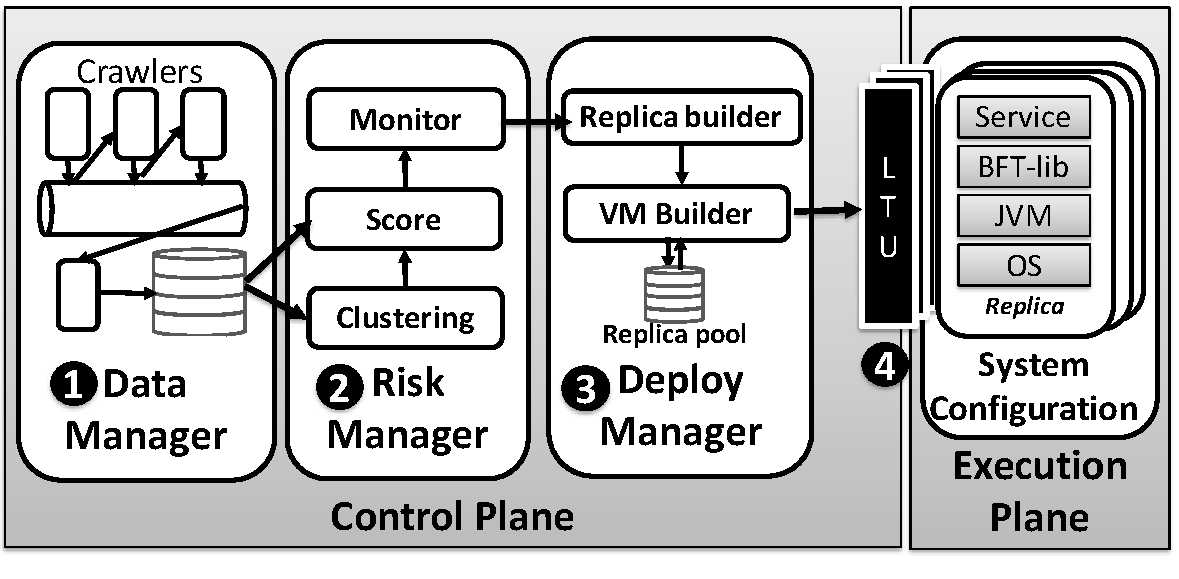
\includegraphics[width=.9\columnwidth]{images/images/architecture_new.pdf}
\vspace{-5mm}
\caption{\system architecture.}
\vspace{-5mm}
\label{fig:arch1}
\end{center}
\end{figure}


\circled{1} \textbf{\fetcher.} \system needs to know the software stack of each available replica to be able to look for vulnerabilities in this software.
The list of software products is provided following the \gls{cpe} Dictionary~\cite{cpe}, which is also used by \gls{nvd}. 
%The \fetcher determines if the CPE list is updated by checking the most recent CPE count in the NVD web page.
For each software, the administrator can indicate the time interval (in years) during which data should be obtained from \gls{nvd}' feeds.

The \fetcher parses the \gls{nvd} feeds considering only the vulnerabilities that affect the chosen products. 
The processing is carried out with several threads cooperatively assemblying as much data as possible about each vulnerability -- a queue is populated with requests pertaining a particular vulnerability, and other threads will look for related data in additional \gls{osint} sources. 
Typically, the other sources are not as well structured as \gls{nvd}, and therefore they have to be handled with specialized HTML parsers that we have developed. 
Currently, the prototype supports five other sources, namely Exploit DB, CVE-details, Ubuntu, Debian, and Microsoft. 
As previously mentioned, such sources provide complementary data, like additional affected products versions not mentioned in \gls{nvd}.

The collected data is stored in a relational database (MySQL).
For each vulnerability we keep its \gls{cve} identifier, the published date, the products it affects, its text description, some \gls{cvss} attributes (e.g., availability and integrity); and exploit and patching dates.


\circled{2} \textbf{\risk.} This component finds out when it is necessary to replace the currently running group of \replicas and discovers an alternative configuration that decreases the risk. 
As explained in Section~\ref{sec:measurerisk}, the risk is computed using score values that require two kinds of data: the information about the vulnerabilities, which is collected by the \fetcher; and the vulnerability clusters. 
A vulnerability cluster is a set of vulnerabilities that are related accordingly to their description (see Section~\ref{sec:details} for details).
The \risk also runs Algorithm~\ref{alg:algorithm2} to monitor the replicated system and trigger reconfigurations.


\circled{3} \textbf{\manager.} 
This component automates the setup and execution of the diverse replicas. 
It creates and deploys the \replicas in the execution environment implementing the decisions of the \risk, i.e., it dictates when and which \replicas leave and join the system. 
We developed a replica builder on top of Vagrant~\cite{vagrant}.
It is responsible for downloading, installing, and configuring the \replicas.
Moreover, it performs replica maintenance, where  \replicas in \QS are booted to carry out automatic software updates (i.e., patching). 


\paragraph{Setup.}
The box configuration is defined in a configuration file, named \emph{Vagrantfile}, consider the example in Listing~\ref{vagrantfile}.
In this file, it is possible to set several options of the box, to name a few:
the box name, the number of CPUs, the amount of memory RAM, the IP, the type of network, sync folders between host and the box, etc. 
Additionally, it is possible to pass some VM-specific parameters, e.g., some CPU/mother board flags such as enabling VT-x technology -- consider the \texttt{modifyvm} fields in Listing~\ref{vagrantfile} (lines 6-14).
It is possible to select different \gls{vm} providers (e.g., libvirt, VMware, VirtualBox, Parallels, Docker, etc), we rely on VirtualBox since it is the one with more diversity opportunities in the Vagrant Cloud~\cite{vagrantcloud}. 
Vagrant Cloud is a website that offers a plethora of different VMs.

\begin{lstlisting}[style=mystyle,caption=Windows Server 2016 Vagrantfile,label=vagrantfile]
Vagrant.configure(2) do |config|
	config.vm.box = "geerlingguy/ubuntu1604"
	config.ssh.insert_key = false
	config.vm.provider "virtualbox" do |v|
		v.customize ["modifyvm", :id, "--cpus", 4]
		v.customize ["modifyvm", :id, "--memory", 22000]
		v.customize ["modifyvm", :id, "--cpuexecutioncap", 100]
		v.customize ["modifyvm", :id, "--ioapic", "on"]
		v.customize ["modifyvm", :id, "--hwvirtex", "on"]
		v.customize ["modifyvm", :id, "--nestedpaging", "on"]
		v.customize ["modifyvm", :id, "--pae", "on"]
		v.customize ["modifyvm", :id, "--natdnshostresolver1", "on"]
		v.customize ["modifyvm", :id, "--natdnsproxy1", "on"]
	end
	config.vm.network "public_network", ip:"192.168.2.50", bridge:"em1"
	config.vm.provision :shell, path: "run_debian.sh", privileged: true
end
\end{lstlisting}

\todo{Add all fields that are mentioned, then add lines to the text}

\paragraph{Download.}
One of the fields of the \emph{Vagranfile} is the boxname, the \texttt{box} field is the key that is used to choose which box will be downloaded, each key is unique for each box.
There are plenty of \glspl{os} and versions ready-to-use, and the same OS/version can have different ``manufacturers" -- some of which are official.

\paragraph{Deploy and provision.}
Vagrant supports complex provisions mechanisms, such as Chef or Puppet, but shell script was sufficient for us. 
This is set in the \emph{Vagranfile} \texttt{provision} field, one can describe the provision steps inline or in an external file and link it to the \emph{Vagranfile}.
Then, when the OS is booting, after the basic setup, the \glspl{os} will execute the provision script.
In this script, we program which software will be downloaded and run in the \glspl{vm} and what configurations are needed. 
We have developed shell scripts for each \glspl{os}, some of which share the same script as Debian and Ubuntu. 
Each \glspl{os}, especially the ones from different \glspl{os} families (e.g., Solaris and BSD) have different commands to execute the same instructions.
Although different, all scripts were meant to do the same thing:
First the script installs the software that is missing in the box -- this is not true for all OSes -- like Java 8, \texttt{wget}, \texttt{unzip}, and any additional software that one wants to install/run after the \glspl{os} boot.



\paragraph{Command and Control.}
There are some simple commands to boot and halt a box, e.g., \texttt{vagrant up} and \texttt{vagrant halt}. 
Vagrant also provides an ssh command (\texttt{vagrant ssh}) that allows the host to connect to the box. 
Our manager component makes the bridge between the \risk and the execution environment.
We developed an API on top of Vagrant, another level of abstraction made to manage replicated systems.


\circled{4} \textbf{LTUs.} Each node that hosts a replica has a Vagrant daemon (see details in next section) running on its trusted domain.
This component is isolated from the internet and communicates only with the \system controller through \gls{tls} channels.

\subsection*{Additional Details}
\label{sec:details}

\textbf{Vulnerability Clustering.}
A few steps are carried out to create the vulnerability clusters. 
First, the vulnerability description needs to be transformed into a vector, where a numerical value is associated with the most relevant words (up to 200 words). 
This operation entails, for example, converting all words to a canonical form and calculating their frequency (less frequent words are given higher weights).
Then, the K-means algorithm is applied to build the clusters~\cite{Jain:2010}, where the number of clusters to be formed is determined by the elbow method~\cite{Thorndike:1953}. 
%Currently, it is set $K=200$.
%The algorithm assigns each vulnerability to the cluster with the minimum distance to the cluster center. 
%Then, it computes the cluster centroid, i.e., the average of each data attribute using only the members of a cluster. 
%Next, it calculates the distance of every vulnerability to the centroid, potentially placing them in close clusters. 
%The algorithm stops when there are no further exchanges between clusters.
%We used the elbow method~\cite{Thorndike53whobelongs} to determine the number of clusters to be formed, in our case was $200$ clusters.
We used the open-source machine learning library Weka~\cite{weka} to build the clusters. 


\subsection*{Clustering}\label{sec:clustering}
Clustering is the process of aggregating elements into similar groups, named clusters. 
For example, two elements from the same cluster have a higher probability of being similar than two elements from different clusters. 
We apply this technique to build clusters of similar vulnerabilities.
One of the benefits of applying clustering techniques to vulnerability-data is that the algorithm does not need prior knowledge about the data.
It is the process alone that discovers the hidden knowledge in the data.
Each cluster is used as a hint that similar vulnerabilities are likely to be activated through the same or similar exploit.
We considered the vulnerability description and published date to find these similarities. 
In the end, it is expected that the clusters have a minimal number of elements that just represent the same or similar vulnerabilities.


In order to apply a clustering technique to our data, we need to follow some steps:

\paragraph{1) Data representation}
We transform the data that is stored in a database into a format that is readable by the clustering algorithm. 
Since we are using Weka~\cite{weka}, the data must be represented as \gls{arff}. 
Basically, this is a CSV file with some meta information, see Listing~\ref{list:arff}.

\begin{lstlisting}[style=mystyle,caption=ARFF file describing a vulnerability.,label=list:arff]
@RELATION vulnerabilities
@ATTRIBUTE cve string
@ATTRIBUTE description string
@ATTRIBUTE published_date date "yyyy-MM-dd"
@DATA
CVE-2017-3301, 'vulnerability in the solaris component of oracle sun systems products suite subcomponent kernel the supported version that is [...] attacks of this vulnerability can result in unauthorized update insert or delete access to some of solaris accessible data cvss v base score integrity impacts', '2017-01-27'
...more
\end{lstlisting}


This file contains all the vulnerabilities entries in the database. 
As we are interested in the vulnerability similarities, we select only the \gls{cve} identifier, the text, that contains the most relevant and nonstructured information, and the published date.
These attributes add meaning and temporal reference to the clustering algorithm.


\paragraph{2) Data preparation}
In general, machine learning algorithms do not handle raw data, then the data needs to be prepared:
First, we transform the \gls{cve} string into a number, basically, for each \gls{cve}, there is a real number that identifies each \gls{cve} unequivocally. 
This attribute is transformed in numeric values using \emph{StringToNominal} filter. 
Each \gls{cve} identifier is mapped to a numeric value.
Second, we transform the published date to a number format that Weka can handle using the \emph{NumericToNominal} filter.
Third, the text description must be transformed into a vector, the vector will represent the frequencies of each word in the whole document of strings. 
We used the \emph{StringToWordVector} to transform a text string into a vector of word weights, these weights represent the relevance of each word in the document.
This filter contains the following parameters:
\begin{itemize}
\item \textbf{TF- and IDF-Transform}, both set to true, TF-IDF stands for term frequency-inverse document frequency. 
This is a statistical measure used to evaluate how relevant a word is to a document in a collection. 
The relevance increases proportionally to the number of times a word appears in the document but is offset by the frequency of the word in the corpus. 
For example, words that appear in all vulnerability descriptions, are less relevant than the ones that appear more in few vulnerabilities.
\item \textbf{lowerCaseTokens}, convert all the words to lower case.
\item \textbf{minTermFreq}, set to -1, this will preserve any word despite their occurrences in the document.
\item \textbf{normalizeDocLength}, set to normalize all data.
\item \textbf{stopwords}, we define a stop word list, then words from this list are discarded. We begin with a general English stop word list containing pronouns, articles, etc. 
\item \textbf{tokenizer}, set to \emph{WordTokenizer}, this filter will remove special characters from the text, there is a default set of characters but we added a few more.
\item \textbf{wordsTopKeep}, is the number of words that will be kept to make the clusters. We kept $200$ as it was the number of words that represent better the lexical of vulnerabilities after removing the \emph{stopwords}.
\end{itemize}


Our goal is to build clusters in such way that similar vulnerabilities, even if they affect different products, are put together in the same cluster. 
For example, recall the vulnerabilities in Table~\ref{tab:missing_products}, which can be put in the same cluster since they are very similar.
Some of the parameters listed above needed some tuning to achieve our goals.
For example, before the tuning, some of the clusters were representing types of vulnerabilities, e.g., buffer overflow, cross-site scripting, etc. 
Since we are not interested in that type of clusters we have refined our \emph{stopword list} to reduce the description vocabulary to contain only what matters for us.
We have done this by iterating the process and checking the most used words (top 200 words) for clustering (this can be seen in Weka's intermediary output).
Then, we added the most relevant from the 200 words that were deviating from our goal.
In the end, we have a stop word list~\footnote{Stop word list is available: here} without the security-vocabulary noise.


When the pre-filtering ends, Weka presents a file very similar to the previous \gls{arff} file with the difference that the features are the most relevant words in the corpus. And each instance contains a value of relevance for each word.


\paragraph{3) Making clusters}
K-means is an unsupervised machine learning algorithm that groups data in K clusters.
The \emph{K-means} has two important parameters: the number of clusters to be formed, we set to $200$ clusters. We used the elbow method~\cite{Thorndike:1953} to decide $k=200$; and the \emph{distance function}, to calculate the distance between objects, the \emph{Euclidean Distance} is the most adequate for this type of data;
The \emph{K-means} computes the distance from each data entry to the cluster center (randomly selected in the first round).
Then, it assigns each data entry to a cluster based on the minimum distance (i.e., Euclidean distance) to each cluster center.
Then, it computes the centroid, that is the average of each data attribute using only the members of each cluster.
Calculate the distance from each data entry to the recent centroids. 
If there is no modification (i.e., re-arrangement of the elements in the cluster), then the clusters are complete, or it recalculates the distance that best fits the elements. 
When the K-means finishes the execution, we take the cluster assignments of each vulnerability. 
The assignments will be added to a new \gls{arff} file, similar to the first one but with a new attribute that is the cluster name (e.g., cluster1, cluster2, etc). 



Sometimes the resulting clusters include vulnerabilities that are unrelated. Therefore, we use the Jaccard index (J-index) to measure the similarity between the vulnerabilities within the cluster. We calculate the J-index of each element, and then the average J-index of the cluster. 
The clusters with a smaller average J-index (below a certain threshold) are considered ill-formed. In this case, we select the vulnerabilities with lower J-index and move them to another cluster that would result in a better J-index. If no such cluster exists, then we create a new one with the ``orphan'' vulnerability.

\textbf{BFT replication.}
Although there has been relevant research on \gls{bft} protocols over the last twenty years, there are few open-source replication libraries that implement them. \system can use any of those libraries, as long as they support replica set reconfigurations.
More specifically, to manage the \replicas, we need the ability to add first a new \replica to the set and then remove the old \replica to be quarantined. 
Therefore, we employ BFT-SMaRt~\cite{Bessani:2014}, a stable \gls{bft} library that provides reconfigurations on the \replicas set.

\textbf{Replica Virtualization.}
\glspl{vm} can be used to implement replicated systems, leveraging on the isolation between the untrusted and the trusted domains~\cite{Sousa:2010,Platania:2014,Distler:2011}.
Recovery triggering can be initiated from the isolated domain in a synchronous manner, reducing the downtime of the service during the reconfigurations. 
In our implementation, we resort to the Vagrant~\cite{vagrant} provisioning tool to do fast deployment of ready-to-use \glspl{os} and applications on \glspl{vm}. 
Vagrant supports several virtualization providers, e.g., VMware and Docker. 
From the available alternatives, we chose VirtualBox~\cite{virtualbox} because it offers more diversity opportunities, i.e., it supports a more extensive set of different guests \glspl{os}.
%The VMs are available in the Vagrant Cloud~\cite{vagrantcloud}.


\section{Evaluation of Replica Set Risk}
\label{sec:diversity}

This section evaluates how \system performs on the selection of dependable \replica configurations.
As discussed in Section~\ref{sec:replica}, we focus our experimental evaluation solely on the OS diversity.
% These play a crucial role in any IT system, and most of the \replica's code is the OS. 
% Thus, they present a high potential to become the most vulnerable part of a \replica.
% Hence, in the following experiments, we explore OS diversity among the replicas. 

In these experiments, we emulate live executions of the system by dividing the collected data into two periods:
(i) a \emph{learning phase} covering all vulnerability data between \emph{2010-1-1} and \emph{2017-9-29}, which is used to setup the \risk's algorithm; and (ii) an \emph{execution phase} composed of the period between \emph{2017-10-1} and \emph{2018-3-30}.
This last period is divided into three intervals of two months (OUT-NOV, DEC-JAN, and FEB-MAR), allowing for three independent tests.
%JAN-FEB, MAR-APR, and MAY-JUN
The goal is to create a knowledge base in the \emph{learning phase} that is used to assess \system choices during each interval of the \emph{execution phase}. 
A run starts on the first day of an interval and then progresses through each day of the interval until the end. Every day, we check if the currently executing replica set could be compromised by an attack exploring the vulnerabilities released on that day. 
We take the most pessimist approach, which is to say that we consider the system to be broken if a vulnerability comes out that affects at least two OSes that would be executing at that time.

Three additional strategies, inspired by previous works, were defined to be compared with \system (Section~\ref{sec:configurations}):

\begin{itemize}
\item \textbf{Equal:} all the replicas use the same randomly-selected OS during the whole execution. 
This strategy corresponds to the scenario where most past \gls{bft} systems have been implemented and evaluated (e.g.,~\cite{Kotla:2010,Aublin:2015,Behl:2015,Veronese:2013,Behl:2017,Liu:2016,Yin:2003,Amir:2011,Bessani:2014,Clement:2009b}). 
Here, compromising a replica would mean an opportunity to intrude the remaining ones.

\item \textbf{Static:} a configuration of $n$ different \glspl{os} is randomly selected, and there are no changes during the whole execution. 
This corresponds to a diverse \gls{bft} system without reconfigurations (e.g.,~\cite{Rodrigues:2001}).

\item \textbf{Random:} a configuration of $n$ \glspl{os} is randomly selected, and at the beginning of each day, a new \gls{os} is randomly picked to replace an existing one. 
This solution represents a system with proactive recovery and diversity, but with no informed strategy for choosing the next \configuration.

%\item \textbf{\system}, $n$ OSes are chosen based the algorithm described in Section~\ref{sec:measurerisk}. This algorithm decides when it is time to replace OSes, which OS is out and which OS is in.
\end{itemize}

The experiments consider a pool of 38 \gls{os} versions to be deployed on four replicas. 
At the beginning of the execution phase, the OSes are assumed to be fully patched.

%\begin{figure}[t]
%\begin{center}
%\includegraphics[width=\columnwidth]{figs/gnuplot/executions/execution.pdf}
%\caption{Compromised system runs over 2 month slots.}
%\label{fig:all_vulns}
%\end{center}
%\end{figure}



\subsection*{Diversity vs Vulnerabilities}
We evaluate how each strategy can prevent the replicated system from being compromised. 
Each strategy is analyzed over $5000$ runs throughout the execution phase in two-month slots. 
Different runs are initiated with distinct random number generator seeds, resulting in potentially different \gls{os} selections over the time slot. 
On each day, we check if there is a vulnerability affecting more than one replica in the current \configuration, and in the affirmative case the execution is stopped.

\begin{figure}[h]
\begin{center}
\includegraphics[width=\columnwidth]{images/gnuplot/executions_new/execution.pdf}
\caption{Compromised system runs over 2 month slots.}
\label{fig:all_vulns}
\end{center}
\end{figure}

\textbf{Results:} Figure~\ref{fig:all_vulns} compares the percentage of compromised runs of all strategies. 
Each bar represents the percentage of runs that did not terminate successfully (lower is better). 
In all three periods, \system presents the best results. 
The \emph{Random} strategy performs worse because eventually, it picks a group of \glspl{os} with common vulnerabilities. 
This result provides evidence for the claim that \system improves the dependability, reducing the probability that $f+1$ \glspl{os} eventually become compromised. 
Interestingly, and contrary to intuition, changing \glspl{os} every day with no criteria will always create unsafe configurations.
Therefore, it is paramount to have selection strategies like the ones we use in \system.
\note{Add all the months we already have}

\subsection*{Risk evaluation}


In order to better understand how \system performed, we isolated one of the $5000$ runs to observe the risk evolution over time. 
We picked the \emph{Random} and \system strategies for this analysis, with results displayed in Figure~\ref{fig:run_all}. 
The graphs present the evolution of the common vulnerabilities, the common clusters, and our risk metric for both schemes. 
Notice that two \glspl{os} might appear in the same cluster but with no mutual flaw as clusters can include many distinct vulnerabilities.

\begin{figure*}[h]
\subfloat[Random]{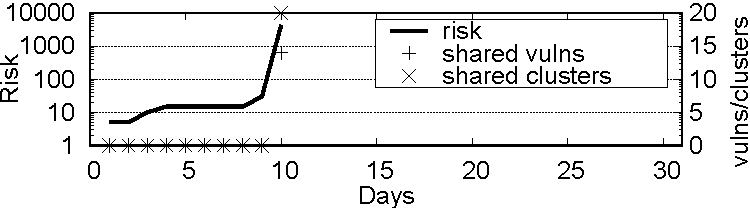
\includegraphics[width=0.5\columnwidth]{images/gnuplot/score/score_random_all.pdf}\label{fig:random_all}}
\hspace{0.5cm}
\subfloat[\system]{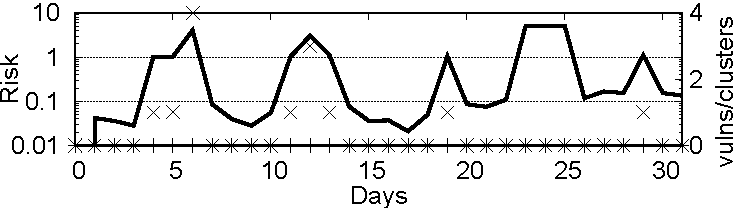
\includegraphics[width=0.5\columnwidth]{images/gnuplot/score/score_final_all.pdf}\label{fig:intel_all}}
\caption{Execution phase for Random and \system OS configuration strategies (log scale).}
\label{fig:run_all}
\end{figure*}

\textbf{Results:} As shown in Figure~\ref{fig:random_all}, \emph{Random} survives only for $10$ days. 
The number of shared clusters and vulnerabilities remains small for the first days. 
Then, there is a replica replacement that adds to the configuration an OS that has common vulnerabilities with the others. 
%Thus, enabling an adversary to compromise enough replicas in the system.

\system survives until the end of the experiment, as the risk is continually managed to keep the system safe. Figure~\ref{fig:intel_all} shows that shared clusters sometimes increase, at the same pace as the risk.
But then, the next reconfigurations are carried out with the goal of decreasing the risk. 
Notice that the risk value is always under $1$ for \system, and in the \emph{Random} is mostly above $10$.


\subsection*{Diversity vs Attacks}

\begin{table}[t]
\begin{center}
{%\small%
\footnotesize
\begin{tabular}{ | p{0.96\columnwidth} | }\hline

\textbf{Samba:} 
\emph{On February 2, 2017, security researchers published details about a zero-day vulnerability in Server Message Block (SMB) of Windows, affecting several versions such as 8.1, 10, Server 2012 R2, and Server 2016. 
Could cause a \gls{dos} condition when a client accesses a malicious SMB.}\\
\textbf{CVES:} 
CVE-2017-0016
\\ \hline

\textbf{Wanna Cry:} 
\emph{On Friday, May 12, 2017, the world was alarmed to discover a widespread ransomware attack that hit organizations in more than 100 countries. Based on a vulnerability in Windows' SMB protocol (nicknamed EternalBlue), discovered by the NSA and leaked by Shadow Brokers.} \\
\textbf{CVES:} 
CVE-2017-0143, CVE-2017-0144, CVE-2017-0145, CVE-2017-0146, CVE-2017-0147, CVE-2017-0148 \\ \hline

\textbf{PowerShell:} 
\emph{Security feature bypass vulnerabilities in Device Guard that could allow an attacker to inject malicious code into a Windows PowerShell session.} \\
\textbf{CVES:}
CVE-2017-0219, CVE-2017-0173, CVE-2017-0215, CVE-2017-0216, CVE-2017-0218\\ \hline

\textbf{Stackclash:} 
\emph{In its 2017 malware forecast, SophosLabs warned that attackers would increasingly target Linux. The flaw, discovered by researchers at Qualys, is in the memory management of several operating systems and affects Linux, OpenBSD, NetBSD, FreeBSD and Solaris.}\\
\textbf{CVES:}
CVE-2017-1000365, CVE-2017-1000366, CVE-2017-1000367, CVE-2017-1000369, CVE-2017-1000370, CVE-2017-1000370, CVE-2017-1000371, CVE-2017-1000372, CVE-2017-1000373, CVE-2017-1000374, CVE-2017-1000375, CVE-2017-1000376, CVE-2017-1000379, CVE-2017-1083, CVE-2017-1084, CVE-2017-3629, CVE-2017-3630, CVE-2017-3631\\ \hline

\end{tabular}
}
\caption{Notable attacks during 2017.}
\label{tab:special_vulns}
\end{center}
\end{table}

This experiment evaluates the strategies when facing notable attacks/vulnerabilities that appeared in $2017$. 
Each attack potentially exploits several flaws, some of which affecting different \glspl{os}. 
The attacks were selected by searching the security news sites for high impact problems, most of them related to more than one CVE. 
As some of the \glspl{cve} include applications, we added more vulnerabilities to the database for this purpose.
Table~\ref{tab:special_vulns} lists the attacks and related \glspl{cve}: Samba,\footnote{https://www.secureworks.com/blog/attacking-windows-smb-zero-day-vulnerability} WannaCry,\footnote{https://securityintelligence.com/wannacry-ransomware-spreads-across-the-globe-makes-organizations-wanna-cry-about-microsoft-vulnerability/} Powershell,\footnote{http://blog.talosintelligence.com/2017/06/ms-tuesday.html} and Stackclash.\footnote{https://nakedsecurity.sophos.com/2017/06/20/stack-clash-linux-vulnerability-you-need-to-patch-now/}


Since some of these attacks might have been prepared months before the vulnerabilities are publicly disclosed, we augmented the execution phase to the full six months. 
As before, the strategies are analyzed over $5000$ runs.


\begin{figure}[t]
\begin{center}
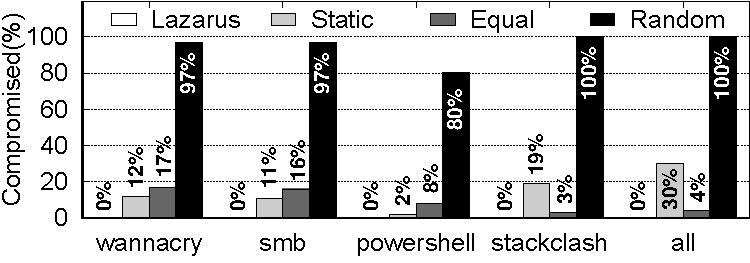
\includegraphics[width=\columnwidth]{images/gnuplot/special_vulns/execution-special.pdf}
\caption{Compromised runs with notable attacks.}
\label{fig:special_vulns}
\end{center}
\end{figure}

\textbf{Results:}
Figure~\ref{fig:special_vulns} shows the percentage of compromised runs for each attack and all attacks put together.
\system is clearly the best at handling the various scenarios, with no compromised executions.
\emph{Random} is the worse, as it does not use any criteria to select the OSes. 
Both \emph{Equal} and \emph{Static} may perform not so bad as they are static, i.e., the \glspl{os} selected by random chance might end up not being exploitable until the end of the run.

\section{Final Remarks}
\label{sec:finalremarkslazarus}

\system addresses the long-standing open problem of evaluating, selecting, and managing the diversity of a \gls{bft} system to make it resilient to malicious adversaries.
Our work focuses on two fundamental issues: how to select the best replicas to run together given the current threat landscape, and what is the performance overhead of running a diverse \gls{bft} system in practice.

